% pumping-lemma-anbn.tex

% !TEX program = pdflatex
\documentclass[tikz]{standalone}
\usepackage{amsmath}
\usepackage{tikz}
\usetikzlibrary{arrows, automata, positioning, decorations.pathmorphing}

\begin{document}
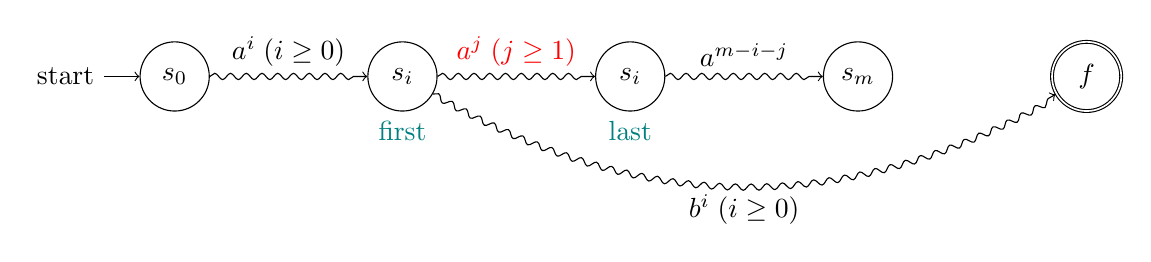
\begin{tikzpicture}[leadsto/.style = {->, decorate, decoration = {snake,
    amplitude = 0.4mm, segment length = 2mm, post length = 1mm}},
    auto, node distance = 2cm]
  \node[state, initial] (init) {$s_{0}$};
  \node[state, right = of init, label = below : {\textcolor{teal}{first}}] (i-first) {$s_{i}$};
  \node[state, right = of i-first, label = below : {\textcolor{teal}{last}}] (i-last) {$s_{i}$};
  \node[state, right = of i-last] (sm) {$s_{m}$};
  \node[state, right = of sm, accepting] (f) {$f$};

  \path (init) edge[leadsto] node[above] {$a^{i}\; (i \ge 0)$} (i-first)
        (i-first) edge[leadsto] node[above] {\textcolor{red}{$a^{j}\; (j \ge 1)$}} (i-last)
        (i-last) edge[leadsto] node[above] {$a^{m-i-j}$} (sm)
        (i-first) edge[leadsto, bend right] node[below] {$b^{i}\; (i \ge 0)$} (f);
\end{tikzpicture}
\end{document}